%%%%%%%%%%%%%%%%%%%%%%%%%%%%%%%%%%%%%%%%%
% Beamer Presentation
% LaTeX Template
% Version 1.0 (10/11/12)
%
% This template has been downloaded from:
% http://www.LaTeXTemplates.com
%
% License:
% CC BY-NC-SA 3.0 (http://creativecommons.org/licenses/by-nc-sa/3.0/)
%
%%%%%%%%%%%%%%%%%%%%%%%%%%%%%%%%%%%%%%%%%

%----------------------------------------------------------------------------------------
%	PACKAGES AND THEMES
%----------------------------------------------------------------------------------------

\documentclass{beamer}

\mode<presentation> {

% The Beamer class comes with a number of default slide themes
% which change the colors and layouts of slides. Below this is a list
% of all the themes, uncomment each in turn to see what they look like.

%\usetheme{default}
%\usetheme{AnnArbor}
%\usetheme{Antibes}
\usetheme{Bergen}
%\usetheme{Berkeley}
%\usetheme{Berlin}
%\usetheme{Boadilla}
%\usetheme{CambridgeUS}
%\usetheme{Copenhagen}
%\usetheme{Darmstadt}
%\usetheme{Dresden}
%\usetheme{Frankfurt}
%\usetheme{Goettingen}
%\usetheme{Hannover}
%\usetheme{Ilmenau}
%\usetheme{JuanLesPins}
%\usetheme{Luebeck}
%\usetheme{Madrid}
%\usetheme{Malmoe}
%\usetheme{Marburg}
%\usetheme{Montpellier}
%\usetheme{PaloAlto}
%\usetheme{Pittsburgh}
%\usetheme{Rochester}
%\usetheme{Singapore}
%\usetheme{Szeged}
%\usetheme{Warsaw}

% As well as themes, the Beamer class has a number of color themes
% for any slide theme. Uncomment each of these in turn to see how it
% changes the colors of your current slide theme.

%\usecolortheme{albatross}
%\usecolortheme{beaver}
%\usecolortheme{beetle}
%\usecolortheme{crane}
%\usecolortheme{dolphin}
%\usecolortheme{dove}
%\usecolortheme{fly}
%\usecolortheme{lily}
%\usecolortheme{orchid}
%\usecolortheme{rose}
%\usecolortheme{seagull}
%\usecolortheme{seahorse}
%\usecolortheme{whale}
\usecolortheme{wolverine}

%\setbeamertemplate{footline} % To remove the footer line in all slides uncomment this line
%\setbeamertemplate{footline}[page number] % To replace the footer line in all slides with a simple slide count uncomment this line

%\setbeamertemplate{navigation symbols}{} % To remove the navigation symbols from the bottom of all slides uncomment this line
}

\usepackage{graphicx} % Allows including images
\usepackage{booktabs} % Allows the use of \toprule, \midrule and \bottomrule in tables
\usepackage{multirow}
\usepackage{adjustbox}
\usepackage{array}
\usepackage{tikz}
\usepackage{soul}
\usetikzlibrary{shapes.geometric, arrows, positioning, fit}
\usepackage[latin1]{inputenc}
\newcommand{\xmark}{\textcolor{red}{\text{\sffamily X}}}
\newcommand{\cmark}{\textcolor{green}{\checkmark}}
\newcommand{\tr}{\text{tr}}
\newcommand{\E}{\textbf{E}}
\newcommand{\diag}{\text{diag}}
\newcommand{\argmax}{\text{argmax}}
\newcommand{\argmin}{\text{argmin}}
\newcommand{\Cov}{\text{Cov}}
\newcommand{\Var}{\text{Var}}
\newcommand{\Vol}{\text{Vol}}
\newcommand{\bx}{\boldsymbol{x}}
\newcommand{\by}{\boldsymbol{y}}
\newcommand{\bX}{\boldsymbol{X}}
\newcommand{\bY}{\boldsymbol{Y}}

%tikz stufff


%----------------------------------------------------------------------------------------
%	TITLE PAGE
%----------------------------------------------------------------------------------------


\title[Informal]{Predicting Human Decision-making in Games}

\author{Charles Zheng} % Your name
\institute[Stanford] % Your institution as it will appear on the bottom of every slide, may be shorthand to save space
{Stanford University}
\date{\today} % Date, can be changed to a custom date

\begin{document}

\begin{frame}
\titlepage % Print the title page as the first slide
\end{frame}


\section{Introduction}

\begin{frame}
\frametitle{History of Chess}
\begin{tabular}{cc}
Shatranj ($\approx$500 AD) & 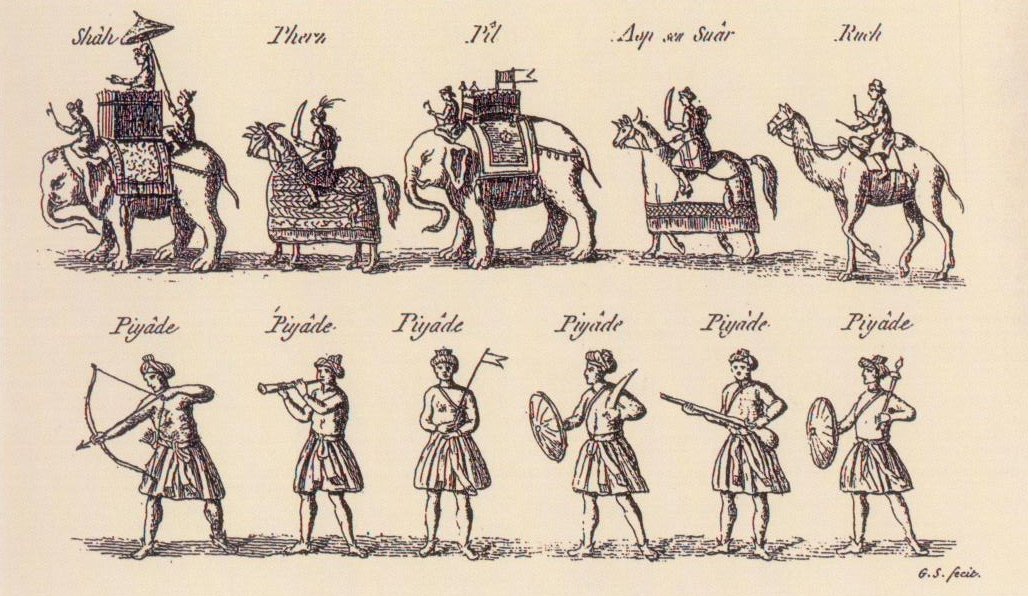
\includegraphics[scale = 0.35]{shatranj.jpg}\\
Chess (1450 AD) & 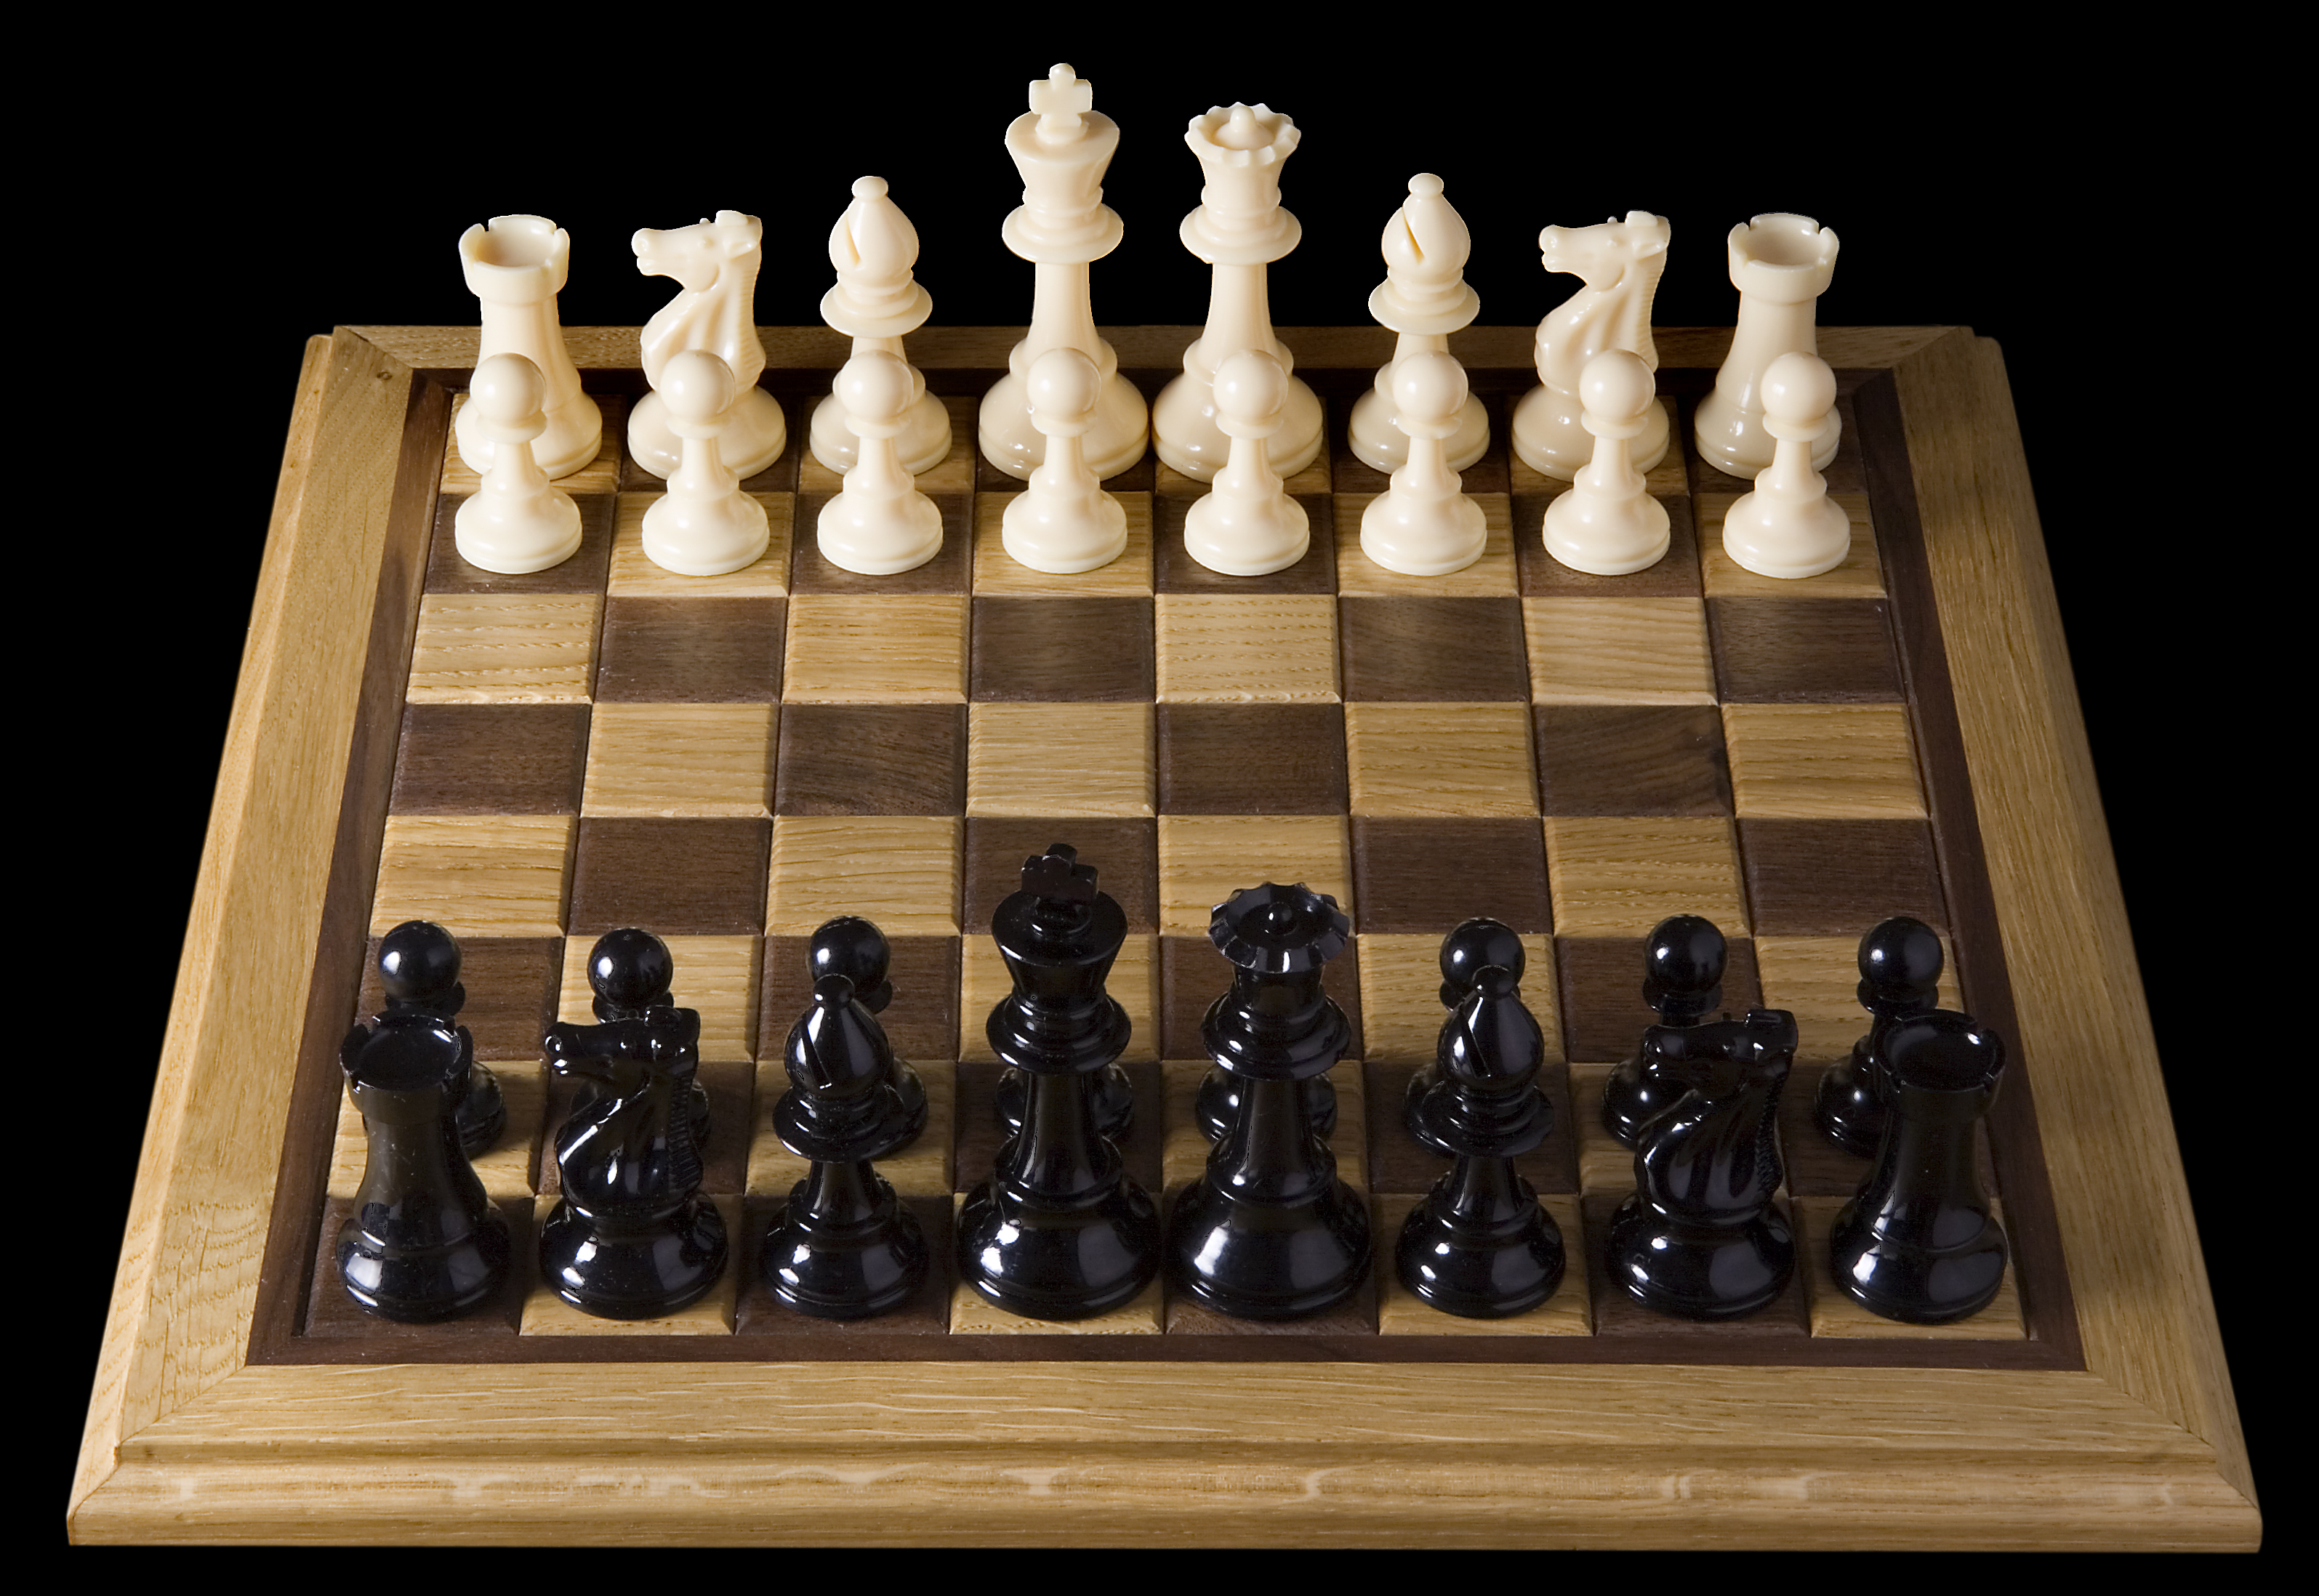
\includegraphics[scale = 0.1]{chess.jpg}\\
Shogi ($\approx$1500 AD) & 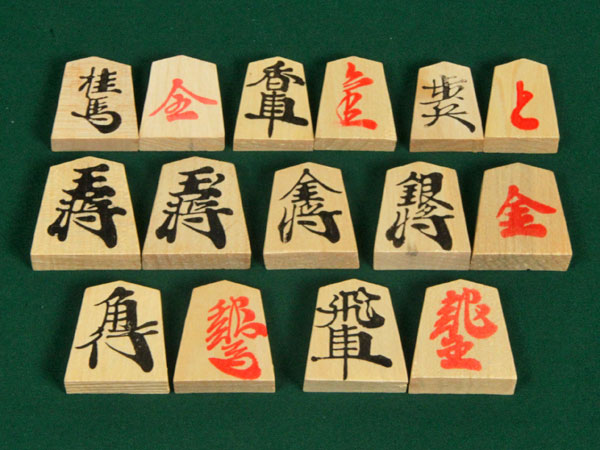
\includegraphics[scale = 0.15]{shogi.jpg}
\end{tabular}
\end{frame}



\begin{frame}
\frametitle{Doubutsu Shogi (Animal Shogi)}
\begin{center}
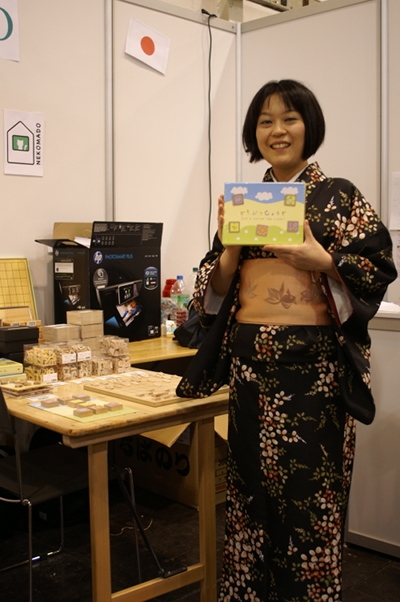
\includegraphics[scale = 0.2]{Madokakitao.jpg}

2009, Madoka Kitao
\end{center}
\end{frame}

\begin{frame}
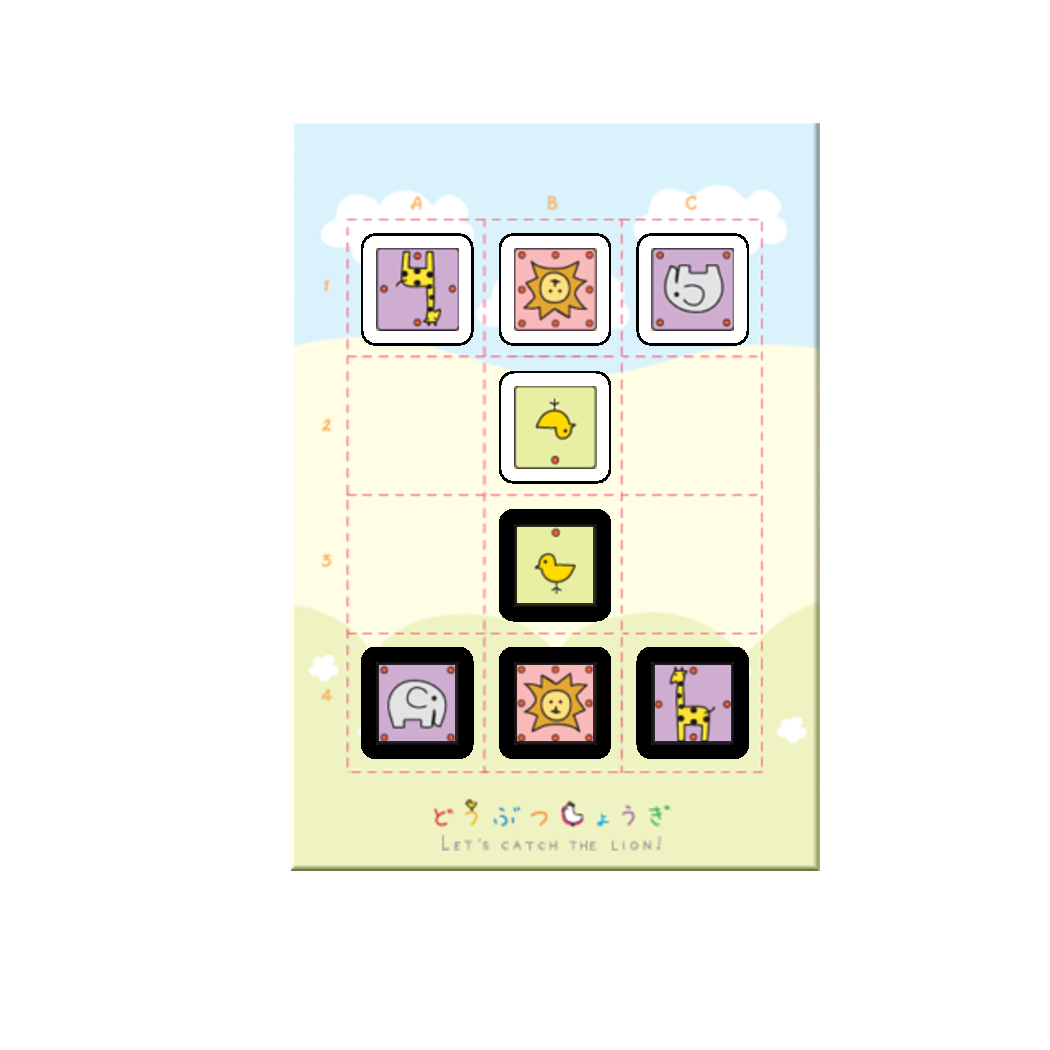
\includegraphics[scale = 0.6, clip=true, trim=1in 1in 0in 0.5in]{example0.pdf}
\end{frame}
\begin{frame}
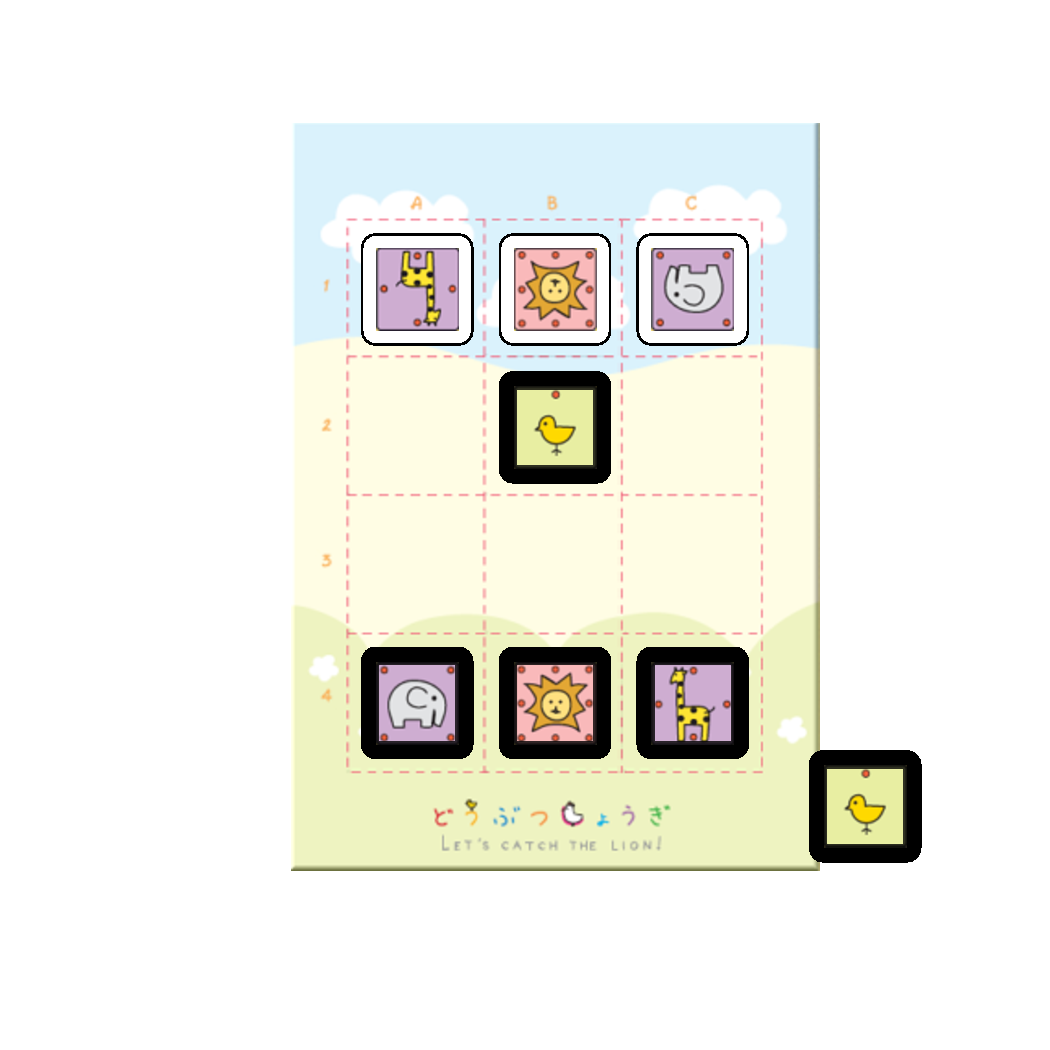
\includegraphics[scale = 0.6, clip=true, trim=1in 1in 0in 0.5in]{example1.pdf}
\end{frame}
\begin{frame}
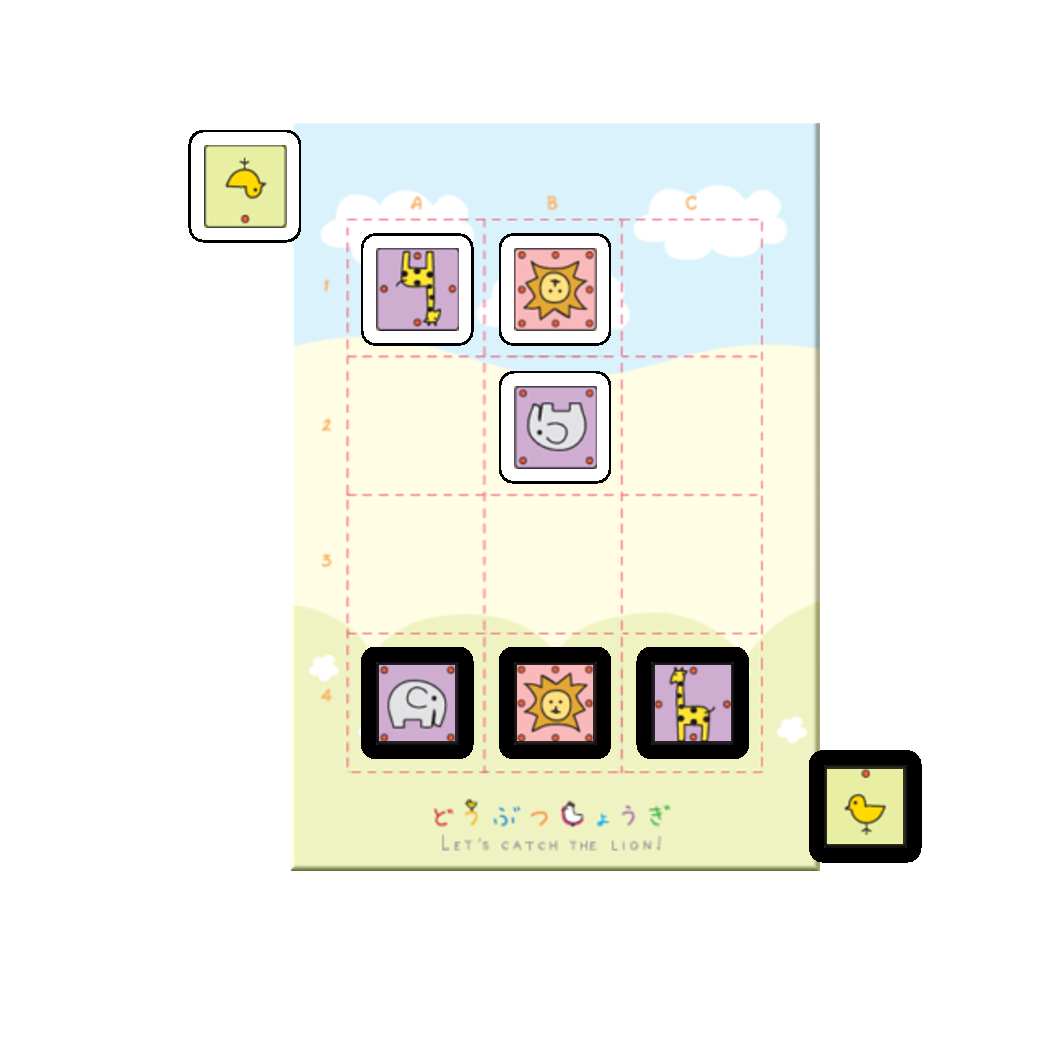
\includegraphics[scale = 0.6, clip=true, trim=1in 1in 0in 0.5in]{example2.pdf}
\end{frame}
\begin{frame}
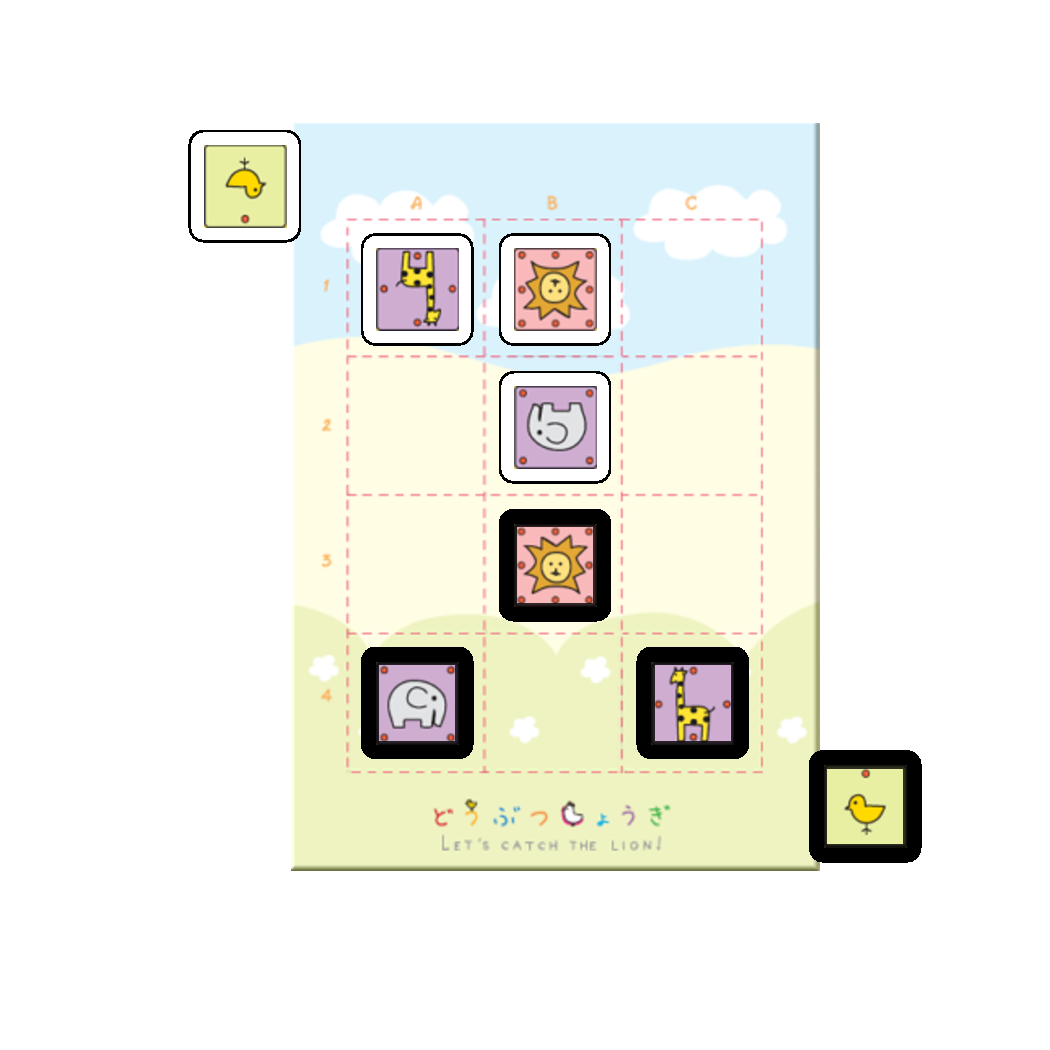
\includegraphics[scale = 0.6, clip=true, trim=1in 1in 0in 0.5in]{example3.pdf}
\end{frame}
\begin{frame}
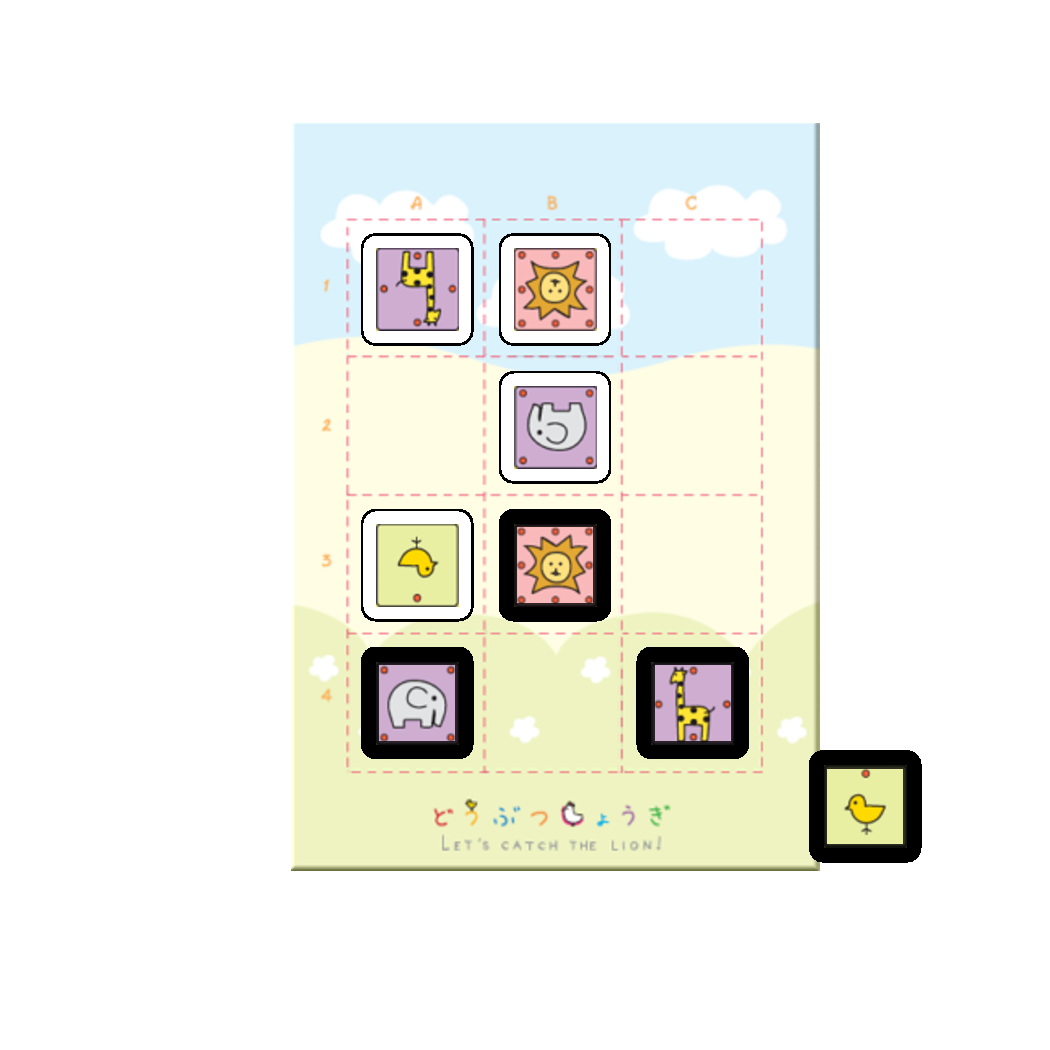
\includegraphics[scale = 0.6, clip=true, trim=1in 1in 0in 0.5in]{example4.pdf}
\end{frame}
\begin{frame}
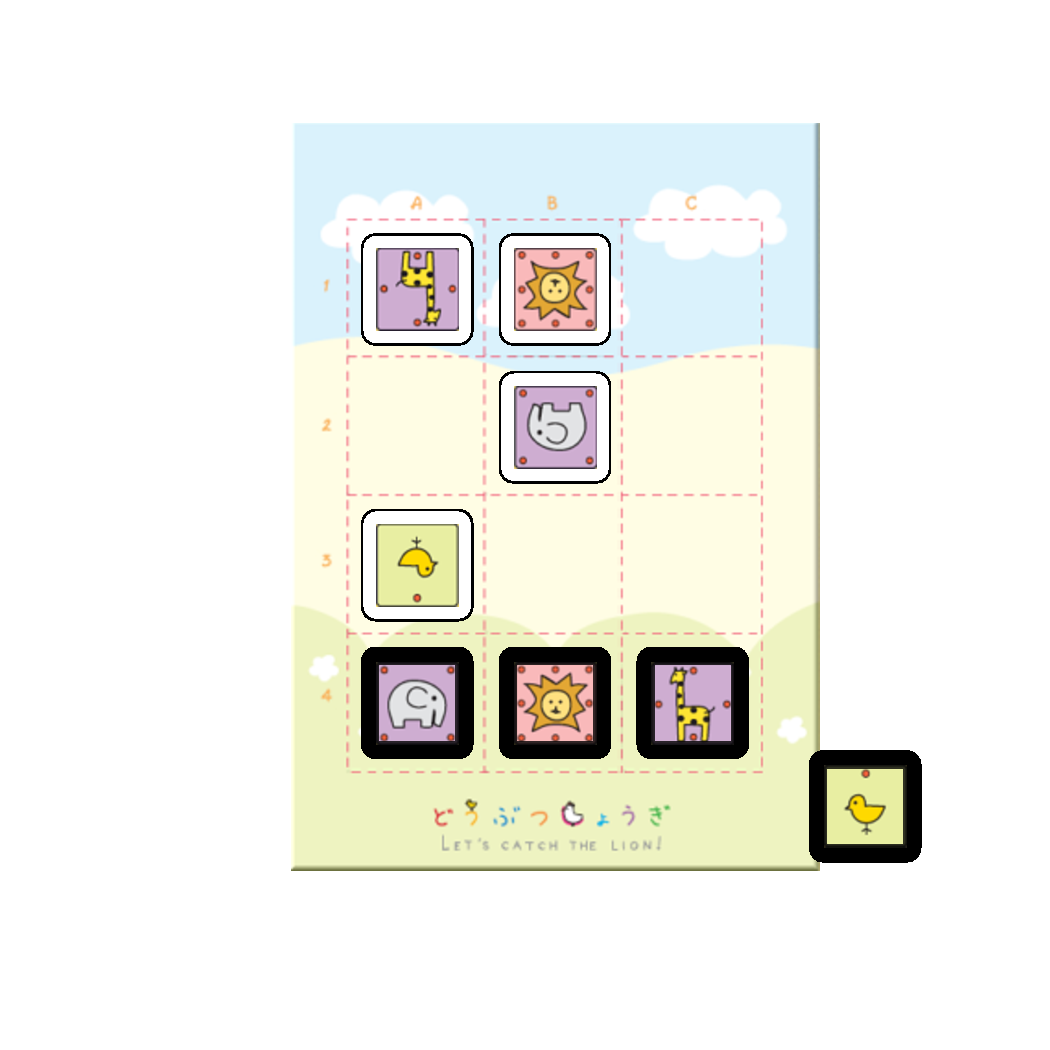
\includegraphics[scale = 0.6, clip=true, trim=1in 1in 0in 0.5in]{example5.pdf}
\end{frame}
\begin{frame}
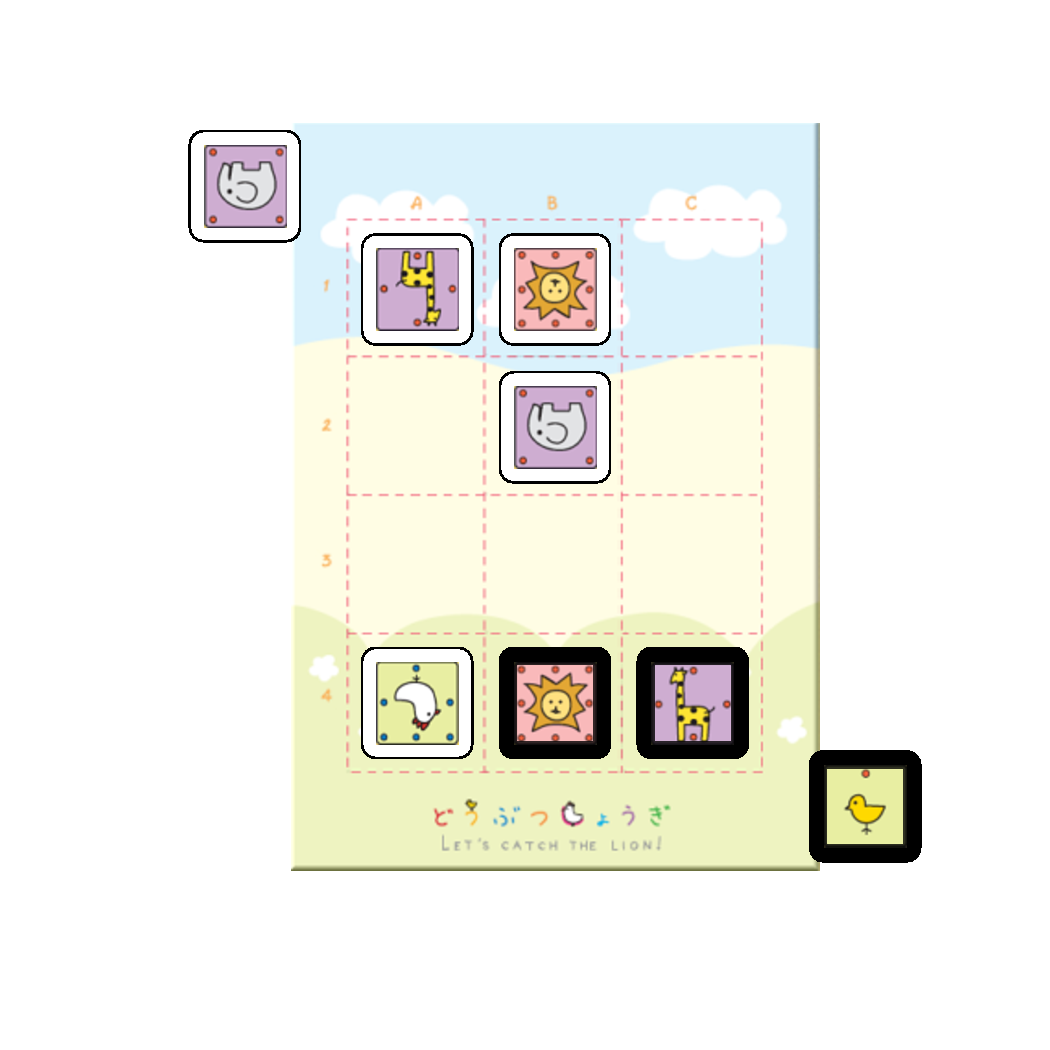
\includegraphics[scale = 0.6, clip=true, trim=1in 1in 0in 0.5in]{example6.pdf}
\end{frame}
\begin{frame}
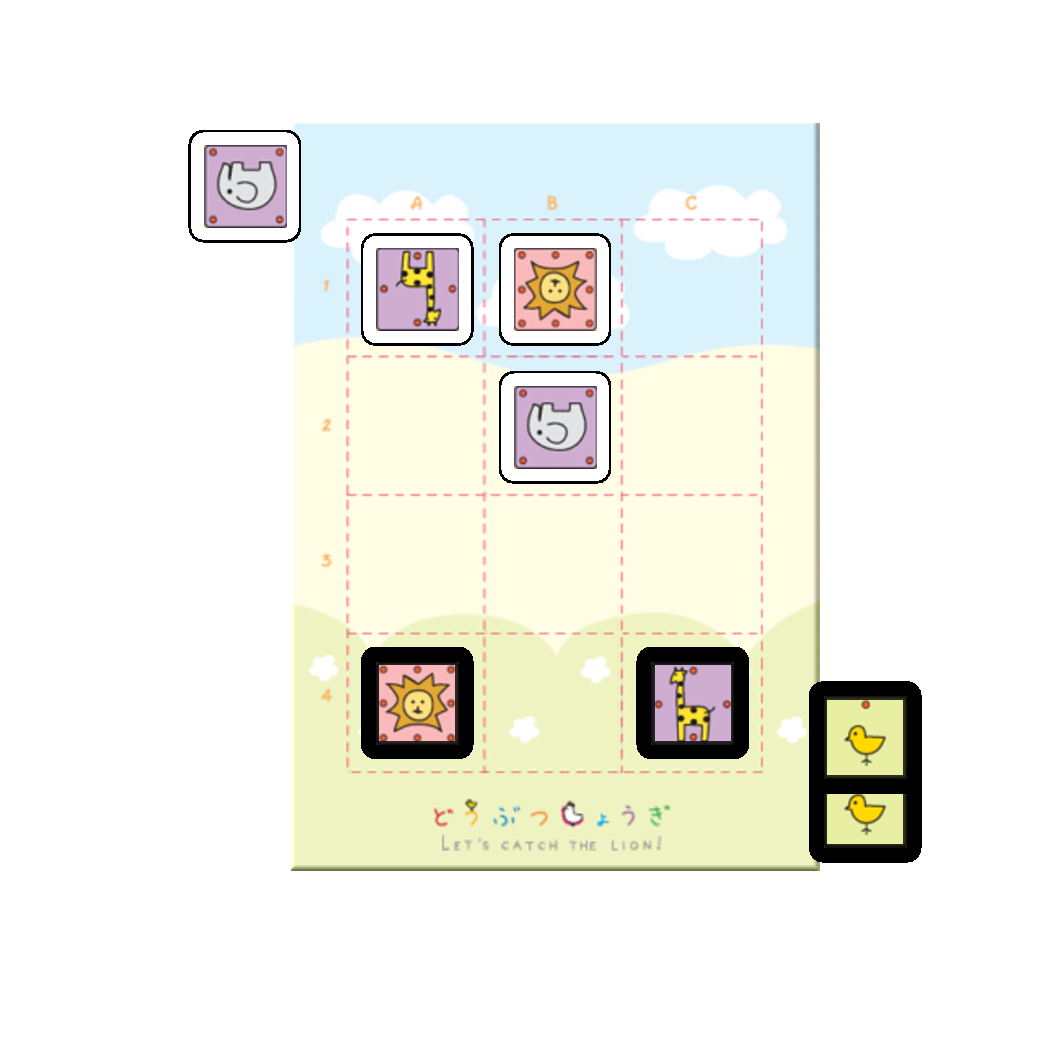
\includegraphics[scale = 0.6, clip=true, trim=1in 1in 0in 0.5in]{example7.pdf}
\end{frame}
\begin{frame}
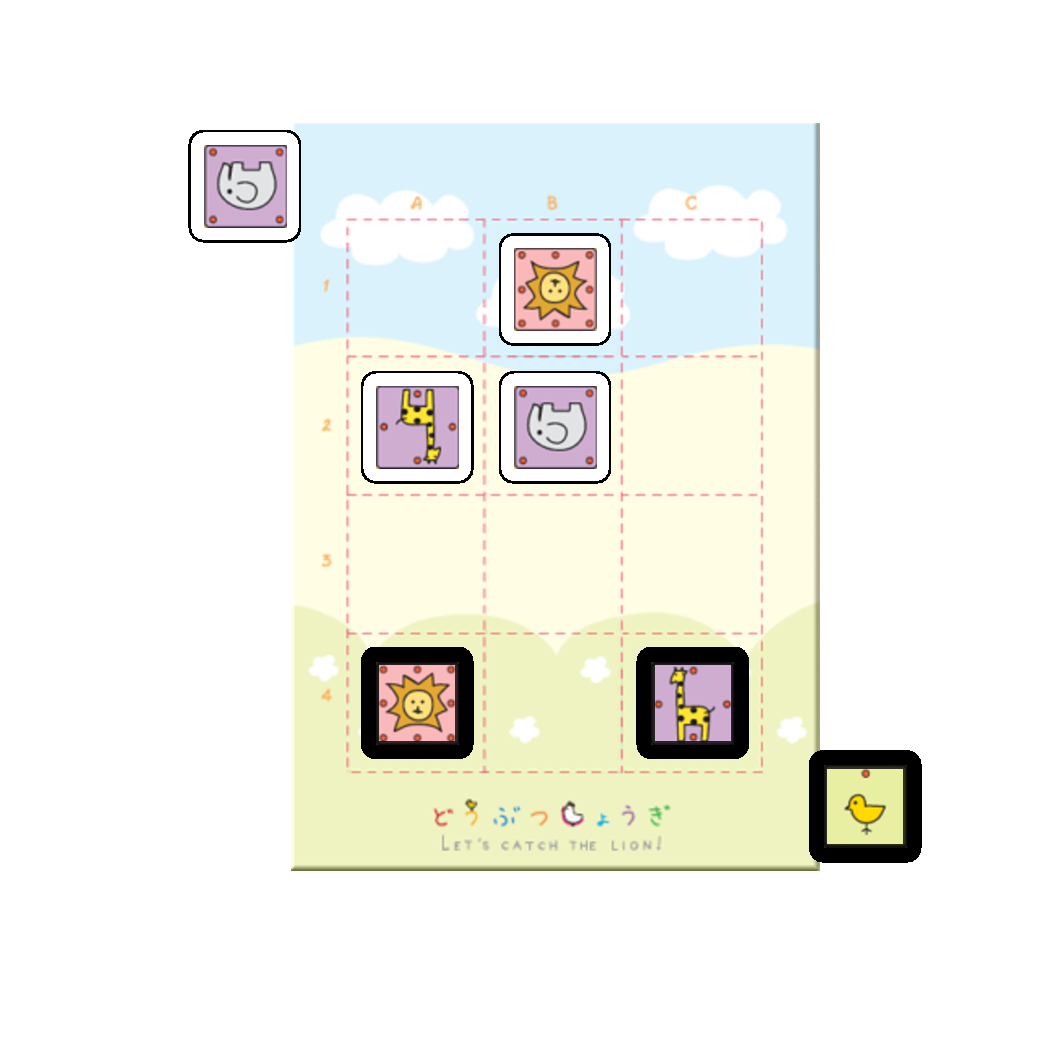
\includegraphics[scale = 0.6, clip=true, trim=1in 1in 0in 0.5in]{example8.pdf}
\end{frame}
\begin{frame}
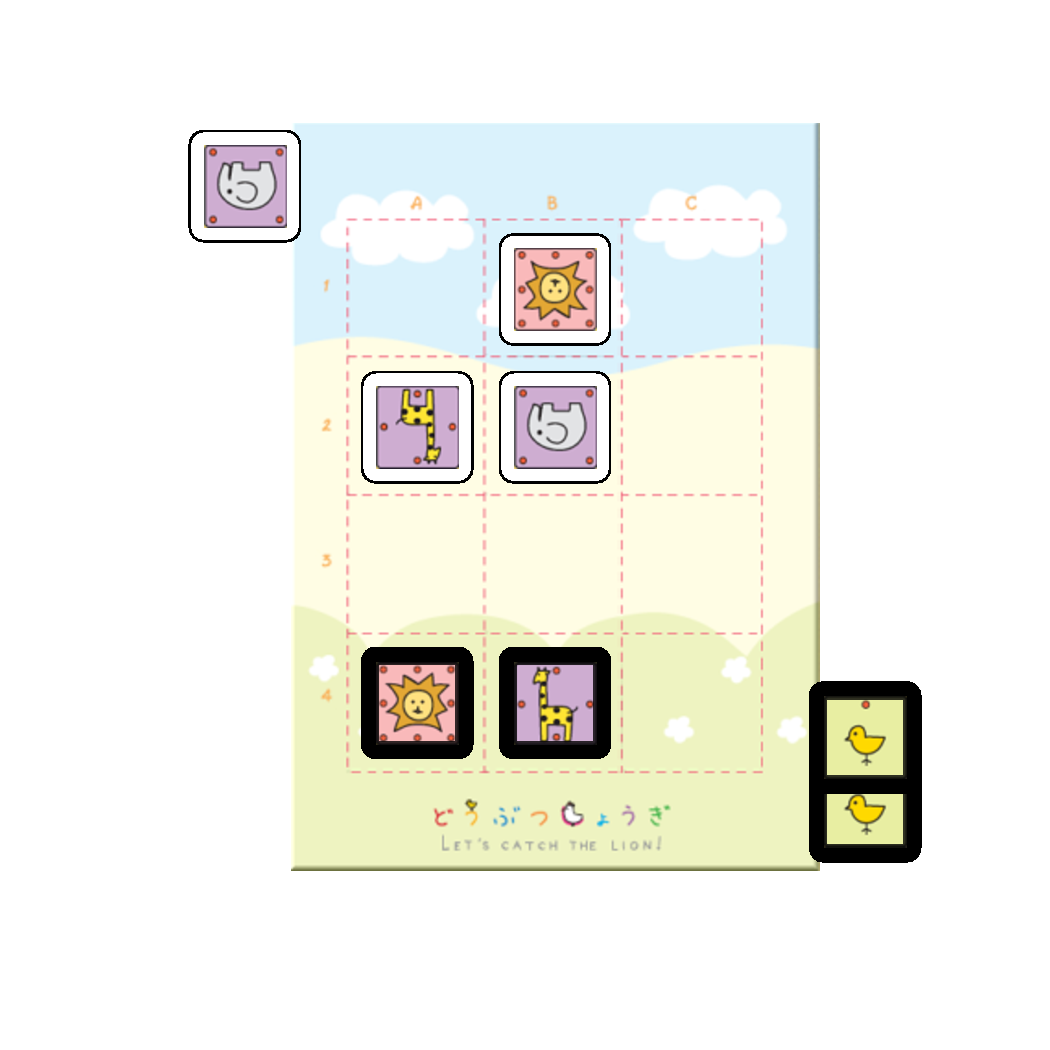
\includegraphics[scale = 0.6, clip=true, trim=1in 1in 0in 0.5in]{example9.pdf}
\end{frame}
\begin{frame}
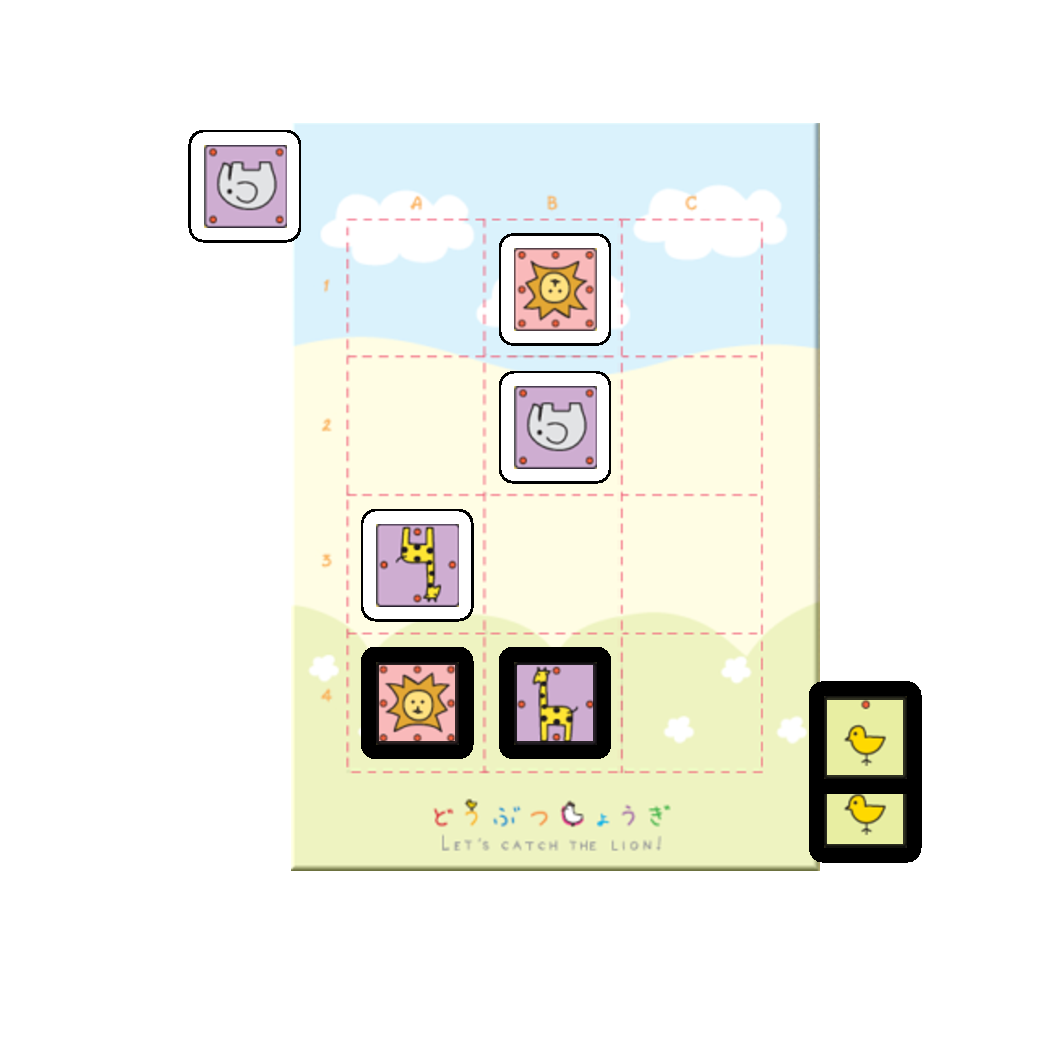
\includegraphics[scale = 0.6, clip=true, trim=1in 1in 0in 0.5in]{example10.pdf}
\end{frame}



\begin{frame}
\frametitle{What is a game?}
\begin{itemize}
\item Set of states $s \in S$.
\item Set of winning states for player 1, $W_1 \subset S$.
\item Winning states for player 2, $W_1 \subset S$.
\item Each state has a set of legal actions $\mathcal{A}(s)$.
\item Player 1 and player 2 take turns choosing the action.
\item A \emph{transition function} $P_a(s, s')$ determines the next state $s'$ resulting from taking action $a$ in states $s$.
\item In \emph{deterministic games}, the transition function equals one for one $s'$ and zero otherwise.
\end{itemize}
\end{frame}

\begin{frame}
\frametitle{Recorded Game Data}
\begin{itemize}
\item List of moves made by both players: "1. Pawn from e2 to e4, 2. Pawn from e7 to e5."
\item Convert to list of \emph{state-action} pairs, $(s_i, a_i)$.
\item $s_i$ is state of game at the beginning of turn $i$, $a_i$ is the move selected at turn $i$.
\end{itemize}
\end{frame}

\begin{frame}
\frametitle{The prediction problem}
\begin{itemize}
\item \emph{Database} of games from players $p_1,\hdots, p_m$ with:
\begin{itemize}
\item Date played
\item Player 1 and player 2 identities
\item List of moves $\to$ player, state, action pairs $(p_j, s_i, a_i)$
\end{itemize}
\item In a \emph{new game}, can we predict which move a given player $p$ will make, given the game state $s$?
\item In other words: given $(p, s)$, guess $a \in \mathcal{A}(s)$.
\end{itemize}
\begin{tabular}{ccc}
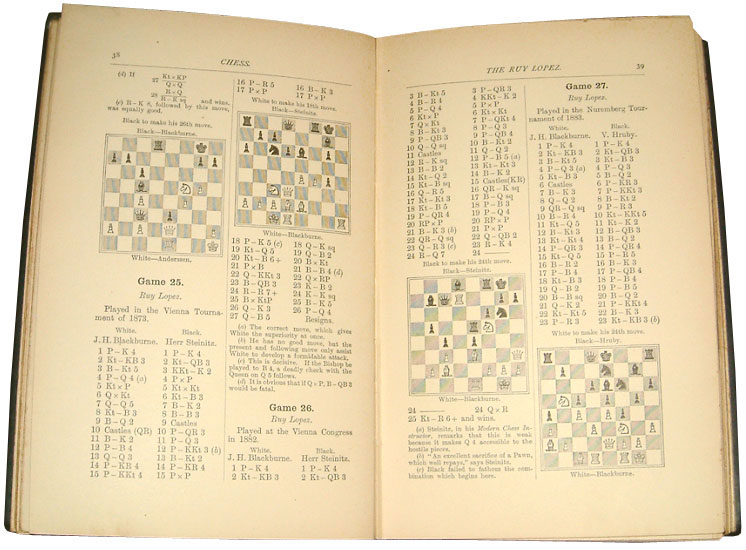
\includegraphics[scale = 0.1]{chessbook.jpg}&
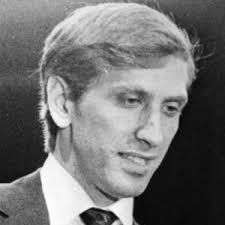
\includegraphics[scale = 0.25]{fisher.jpeg}&
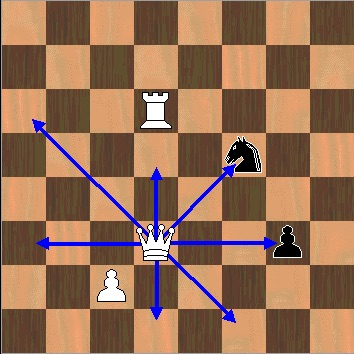
\includegraphics[scale = 0.2]{Queenmoves3.jpg}
\end{tabular}
\end{frame}

\begin{frame}
\frametitle{Motivation}
\begin{itemize}
\item First step for building superhuman AI player
\item Detecting computer-aided cheating (Regan 2013)
\item Objectively evaluating professional players (Matej 2011)
\item Betting on results of professional games?
\item Writing a book about `most common chess mistakes' 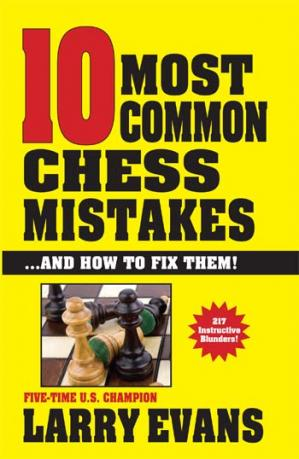
\includegraphics[scale = 0.2]{chess_mistakes.jpg}
\item Use machine learning to learn about human learning (?)
\end{itemize}
\end{frame}


\section{Methods}

\begin{frame}
\sectionpage
\end{frame}

\begin{frame}
\frametitle{Features}
\begin{itemize}
\item In order to apply machine learning, need numeric features for the state $s$.
\item Let $x_1(s),\hdots, x_p(s)$ denote the features, $\vec{x}(s)$=feature vector.
\item Borrow features from chess programming: material, board control, king safety, etc.?
\item Or try to do generic \emph{feature selection} or \emph{representation learning}?
\end{itemize}
\end{frame}

\begin{frame}
\frametitle{Features}
We use a minimalistic featurization.  The 3x4 board is converted into a 136-length binary vector.\vspace{0.5in}

\begin{tabular}{c|c}
\hline
$x_1$ & Player 1 has a king at (1,1)?\\ \hline
$x_2$ & Player 1 has a rook at (1,1)?\\ \hline
$x_{23}$ & Player 2 has a bishop at (1, 3)?\\ \hline
$x_{132}$ & Does player 1 have two rooks in hand? \\\hline
\end{tabular}
\vspace{0.5in}

We also consider \emph{second-order interactions}: e.g. $x_4x_{23}$ = Does player 1 have a pawn on (1,1) and player 2 have a bishop on (1, 3)?

\end{frame}


\begin{frame}
\frametitle{Policy model}
\begin{itemize}
\item Fit the model
\[
\Pr[A = a|s] = \frac{\exp[\beta_a^T \vec{x}(s)]}{\sum_{a \in \mathcal{A}} \exp[\beta_a^T \vec{x}(s)]}.
\]
where $\mathcal{A}$ is the set of \emph{all possible moves} in the game (not just legal moves in $s$).
\item When \emph{predicting}, choose the action with the highest predicted probability among \emph{legal} actions
\[
\hat{A}(s) = \max_{a \in \mathcal{A}(s)} \beta_a^T \vec{x}(s).
\]
\end{itemize}
\end{frame}

\begin{frame}
\frametitle{Policy and values}
\begin{itemize}
\item A policy $\pi(s, a)$ specifies a probability distribution of \emph{actions} for each state $s \in S$.
\item The value of a state $V^{\pi_1,\pi_2}(s)$ is the probability that player 1 wins if player 1 uses policy $\pi_1$
and player 2 uses policy $\pi_2$.
\[
V^{\pi_1,\pi_2}(s) = \begin{cases}
1 &\text{ if }s\in W_1\\
0 &\text{ if }s \in W_2\\
& \sum_{a \in \mathcal{A}} \pi_i(s, a) \sum_{s'} P_a(s, s') V^{\pi_1,\pi_2}(s')
\end{cases}
\]
where $i=1$ if it's player 1's turn and $i=2$ if it's player 2's turn.
\end{itemize}
\end{frame}

\begin{frame}
\frametitle{Evaluation functions}
\begin{itemize}
\item In a deterministic game, let $s'(s, a)$ denote the state with probability 1 resulting from $(s, a)$
\item Suppose player 1 knows player 2's policy.  Then it would be rational for player 1 to choose $a$ which maximizes the 
\[
V^{\pi_1,\pi_2}(s'(s, a)).
\]
\item However, humans are not perfectly rational nor omniscient.  Perhaps players have an intuitive \emph{evaluation function} $E$ which approximates the true value function,
\[
E(s) \approx V^{\pi_1,\pi_2}(s).
\]
\end{itemize}
\end{frame}

\begin{frame}
\frametitle{Evaluation model}
\begin{itemize}
\item Suppose a player does have a mental evaluation function $E$.  Should they always choose $a$ which maximizes $E(s'(s, a))$?
\item Even in deterministic games, there is an advantage to being unpredictable!
\item This leads to a multinomial model of player choice:
\[
\Pr[A = a|s] = \frac{\exp[E(s'(s, a))]}{\sum_{a' \in \mathcal{A}(s)} E(s'(s, a'))}
\]
Note that $E(s)$ need not be a probability: it could be a real number.
Real-valued $E(s)$ may be more realistic, anyways.
\end{itemize}
\end{frame}

\begin{frame}
\frametitle{How to fit the evaluation model?}
\begin{itemize}
\item For fixed player $p$, let $\{(s_i, a_i)\}_{i=1}^n$ denote all the state-action pairs for that player in the database.
\item Fit a logistic evaluation model, minimizing the loss
\[
\sum_{i=1}^n \vec{x}(s'(s_i, a_i))^T \beta - \log(\sum_{a \in \mathcal{A}} \exp[\beta^T \vec{x}(s'(s_i, a))]).
\]
\item Loss function is convex!
\item For large feature models, recommended to use L1 and L2 regularization.
\item To predict, choose $a \in \mathcal{A}$ maximizing $\beta^T s'(s, a)$.
\end{itemize}
\end{frame}

\section{Data}

\begin{frame}
\sectionpage
\end{frame}

\begin{frame}
\frametitle{Doubutsu Shogi on LittleGolem}
\begin{itemize}
\item Data obtained from {\tt littlegolem.com}, a free turn-based game site, using {\tt scrapeR}
\item 85 players, 727 games, 17094 turns (state-action pairs)
\item Oct 2012 to Apr 2016
\item Usernames have been anonymized
\end{itemize}
\begin{center}
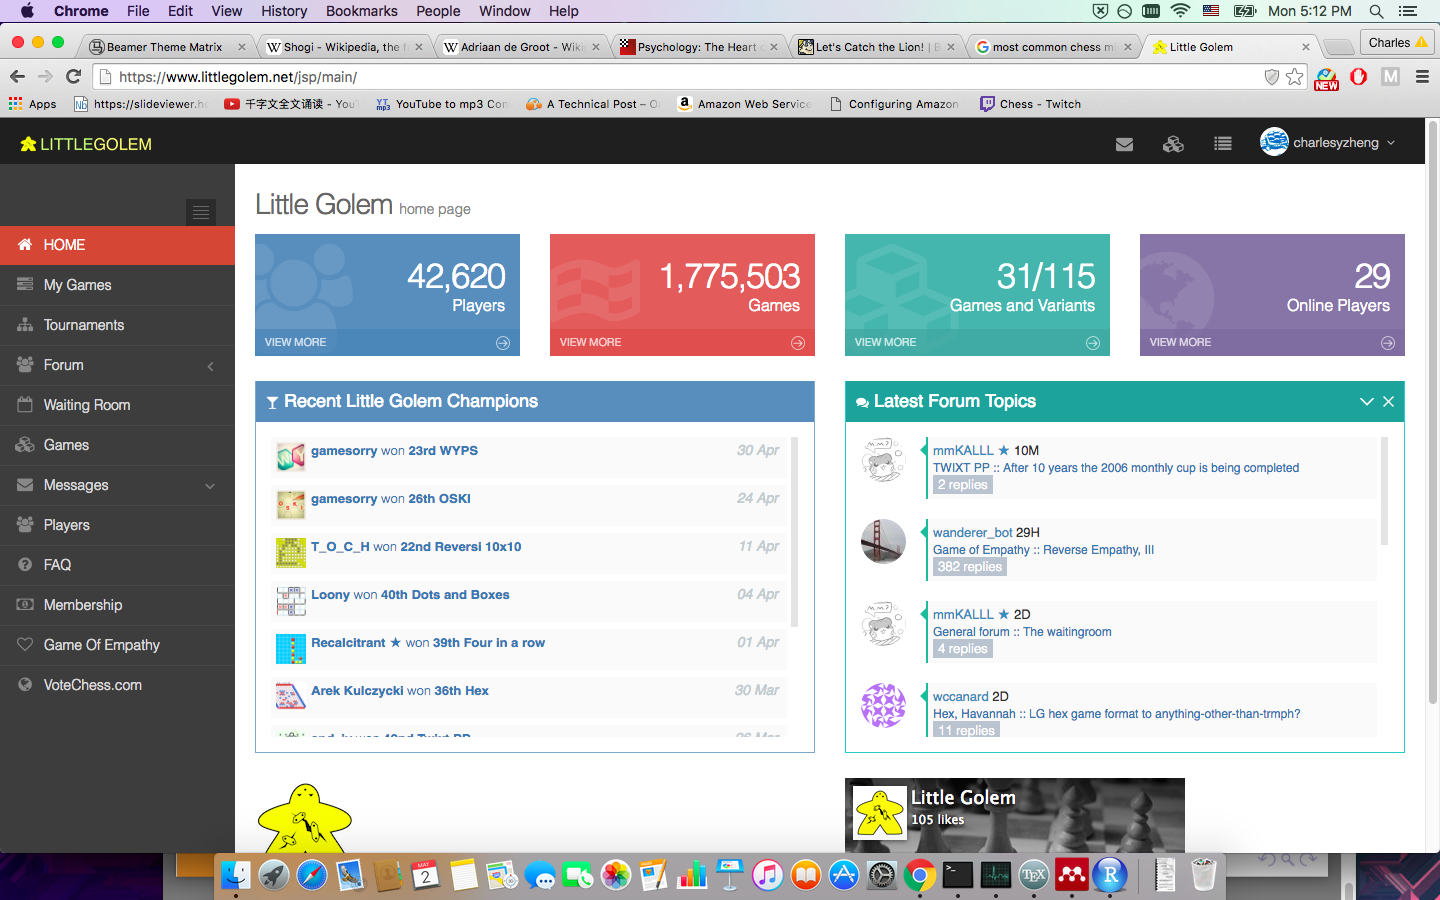
\includegraphics[scale = 0.1]{lg.png}
\end{center}
\end{frame}

\end{document}






